\documentclass{amsart}

\input{../preamble_general.tex}

%\author{Jalen Chrysos}
\title{Practice Midterm 2}

% topics:
% induction
% counting 
% induced subgraphs
% graph isomorphism, "triangle free"
% graph score and Havel-Hakimi
% K_n, K_{m,n} and C_n
% connected components
% graph distance
% 2-connected graphs, ear decomposition

% leaf lemma
% Cayley's formula
% contracting edge of a tree

% K_5 and K_{3,3} are non-planar
% V - E + F = 2 for planar graphs
% 


\begin{document}
	
	\maketitle 
	
	\textit{In all questions, please justify your answers as appropriate. Any legitimate solution will be accepted, unless the question specifically calls for a certain method.}\\
	
	\noindent \textbf{Question 1}: In each part, produce a graph with the described property, or show that none exists.
	
	\begin{enumerate}[(a)]
		\item A tree such that every vertex has degree $\geq 2$. \vspace{170pt}
		
		\item Two trees, each with 5 vertices, which are non-isomorphic. \vspace{170pt}
		
		\item A triangle-free graph that is not 2-colorable.\vspace{170pt}
		
		\item A plane graph with at least 3 faces, all of which have exactly 3 sides. \vspace{150pt}
		
		\item A non-planar connected graph containing no subgraph isomorphic to $K_5$ or $K_{3,3}$.\vspace{170pt}
		
		\item A simple plane graph whose dual is not simple \textit{(recall that simple means that every two vertices have at most one edge between them and no edge connects a vertex to itself)}.\vspace{170pt}
		
		\item A plane graph whose faces all have exactly 3 sides, which contains $C_4$ as an induced subgraph.
	\end{enumerate}
	
	\newpage 
	
	\noindent \textbf{Question 2}: Please do not use the Matrix Tree Theorem in this question.
	
	\begin{enumerate}[(a)]
		\item Compute the number of spanning trees of the graph pictured below:
		
		\begin{figure}[h]
			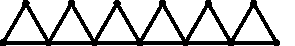
\includegraphics{./Asymptote_Figs/6Triangles.pdf}
		\end{figure}
		
		\vspace{230pt}
		
		\item Let $e$ be an edge in $K_n$. How many spanning trees of $K_n$ include $e$? \vspace{250pt}
	\end{enumerate}
	
	\newpage
	\noindent \textbf{Question 3}: A soccer ball maker stitches together polygonal patches to make a ball. You can assume that a patch cannot neighbor itself, and two patches share at most one edge.
	\begin{enumerate}[(a)]
		\item First, he makes a ball from $p$ pentagonal patches. What is the least value of $p$ for which this is possible? \vspace{250pt}
		\item Next, he makes a ball from $h$ hexagonal patches and $p$ pentagonal patches, such that \textit{exactly 3 patches meet at each vertex}. Show that there is only one possible value of $p$ where this is possible, and determine this value. (\textit{Hint: Compute $V$, $E$, and $F$ in terms of $h$ and $p$}).
	\end{enumerate}
	
	\newpage 
	
	\noindent \textbf{Question 4}: 
	
	\begin{enumerate}[(a)]
		\item Using the Matrix Tree Theorem, produce a matrix whose determinant corresponds to the number of spanning trees of $K_{3,3}$. \vspace{200pt}
		
		\item Compute this determinant by row reduction and verify that it is 81. \textit{(If you don't want to do this, you can skip to part (c))}.\vspace{200pt}
		
		
		\item What is the least number of spanning trees that a connected non-planar graph can have?
	\end{enumerate}
	
\end{document}